\begin{figure}
    \centering
    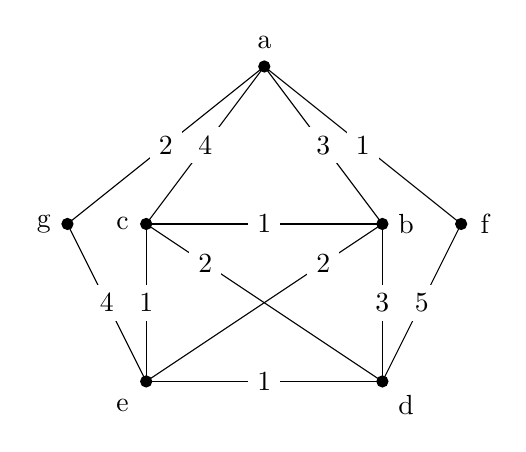
\begin{tikzpicture}

%% vertices
\draw[fill=black] (2.5,4) circle (2pt); %% a
\draw[fill=black] (4,2) circle (2pt);   %% b
\draw[fill=black] (1,2) circle (2pt);   %% c
\draw[fill=black] (4,0) circle (2pt);   %% d
\draw[fill=black] (1,0) circle (2pt);   %% e
\draw[fill=black] (5,2) circle (2pt);   %% f
\draw[fill=black] (0,2) circle (2pt);   %% g

%% vertex labels
\node at (2.5,4.3) (a){a};
\node at (4.3,2) (b){b};
\node at (0.7,2) (c){c};
\node at (4.3,-0.3) (d){d};
\node at (0.7,-0.3) (e){e};
\node at (5.3,2) (f){f};
\node at (-0.3,2) (g){g};

%%% edges
\draw (2.5,4) -- (4,2) node [midway, fill=white] {3};   %% ab
\draw (2.5,4) -- (1,2) node [midway, fill=white] {4};   %% ac
\draw (4,2) -- (1,2) node [midway, fill=white] {1};     %% bc
\draw (4,2) -- (4,0) node [midway, fill=white] {3};     %% bd
\draw (4,2) -- (1,0) node [near start, fill=white] {2}; %% be
\draw (1,2) -- (4,0) node [near start, fill=white] {2}; %% cd
\draw (1,2) -- (1,0) node [midway, fill=white] {1};     %% ce
\draw (4,0) -- (1,0) node [midway, fill=white] {1};     %% de
\draw (2.5,4) -- (5,2) node [midway, fill=white] {1};   %% af
\draw (4,0) -- (5,2) node [midway, fill=white] {5};     %% df
\draw (2.5,4) -- (0,2) node [midway, fill=white] {2};   %% ag
\draw (1,0) -- (0,2) node [midway, fill=white] {4};     %% eg
    \end{tikzpicture}
    \label{question1}
    \caption{Graph in question 1}
\end{figure}